
\begin{figure*}[p]%
 \centering
 \subfloat[Preview the Rotation Angle]{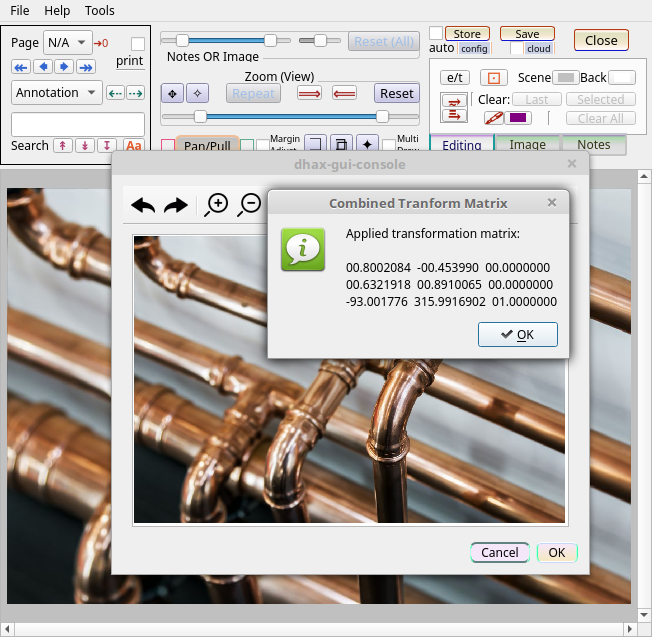
\includegraphics[width=0.51\textwidth, 
trim=0cm 2cm 0cm 2cm, clip]{gui/angle.png}\label{fig:a}}\hspace*{1em}%
 \subfloat[Initiate a Color-Mask]{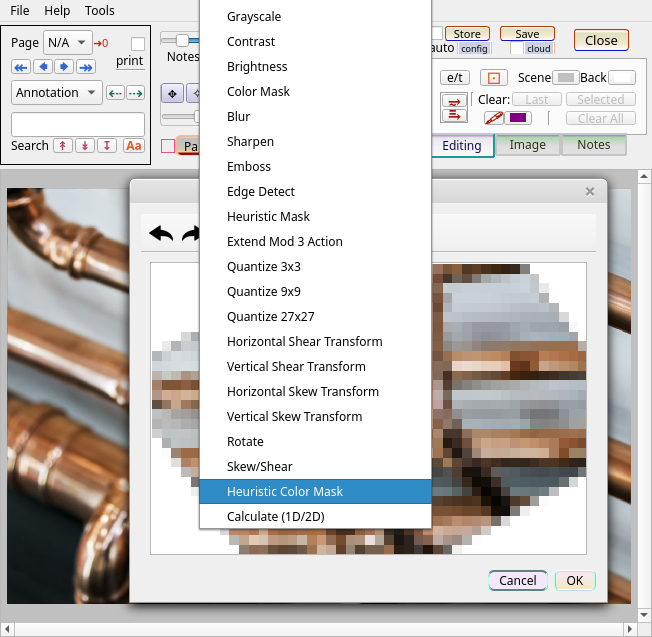
\includegraphics[width=0.51\textwidth, 
trim=0cm 7mm 0cm 47mm, clip]{gui/mask.png}\label{fig:b}}\\
 \subfloat[Select a Color for the Mask]{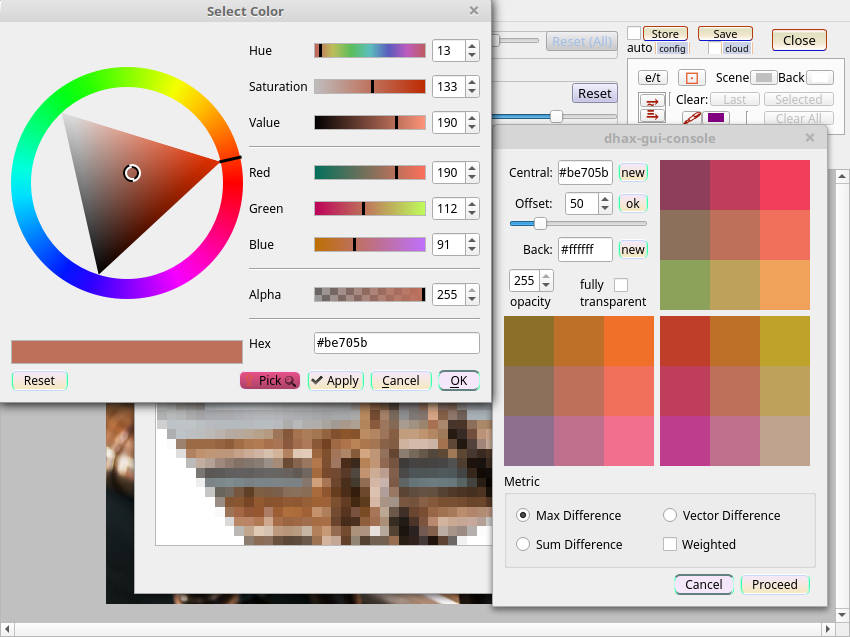
\includegraphics[width=0.51\textwidth]{gui/choose.png}\label{fig:c}}\hspace*{1em}%
 \subfloat[Request Foreground Calculations]{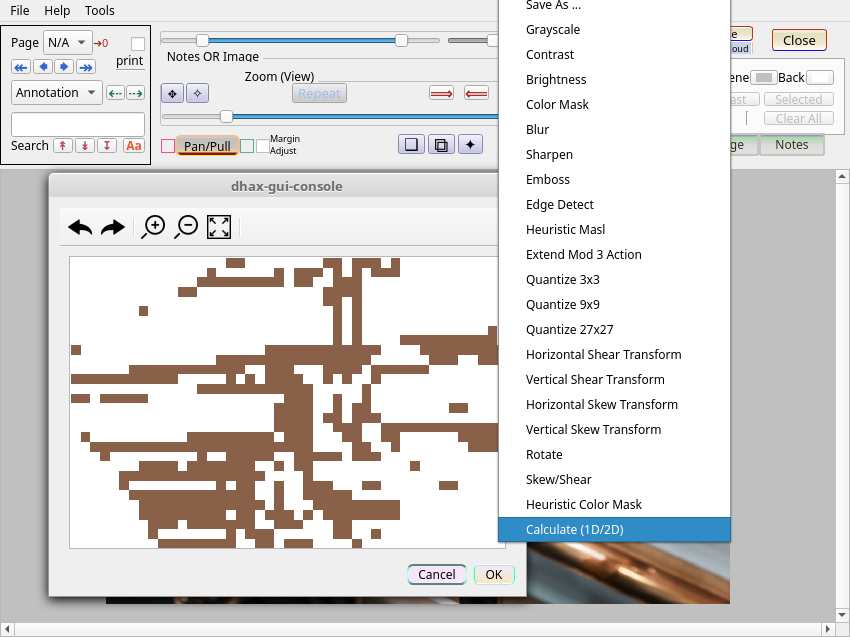
\includegraphics[width=0.51\textwidth]{gui/calc.png}\label{fig:d}}\\
 \subfloat[threshold]{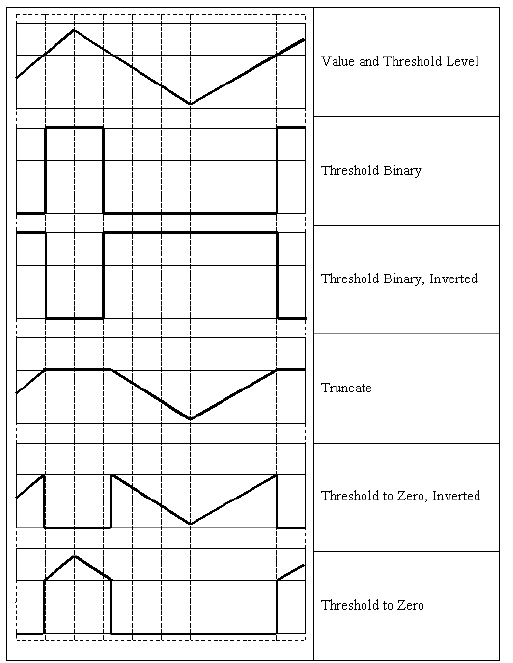
\includegraphics[width=0.51\textwidth]{gui/threshold.png}\label{fig:e}}\hspace*{1em}%
 \subfloat[total]{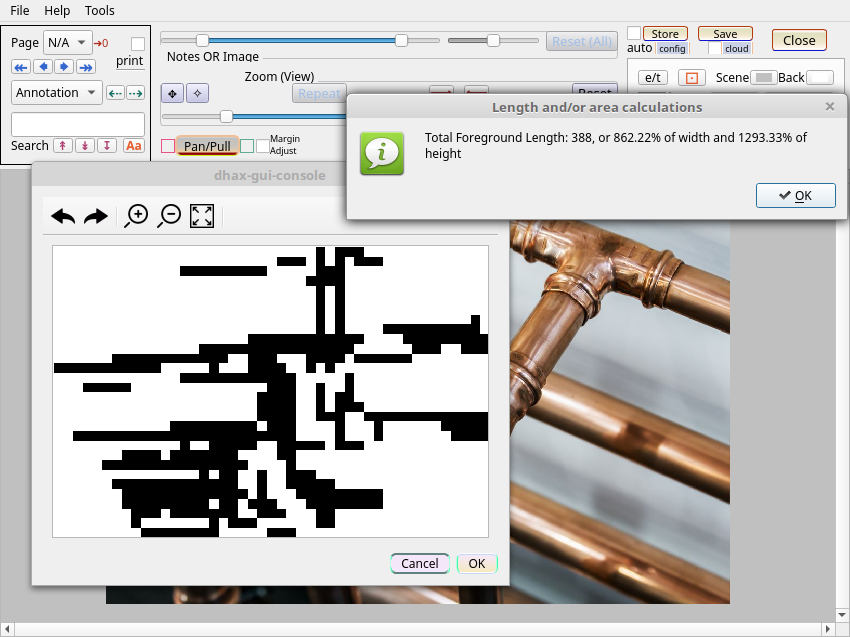
\includegraphics[width=0.51\textwidth]{gui/total.png}\label{fig:f}}\\
 \caption{An Interactive Workflow with XCSD}%
 \label{fig:all}%
{\labelbox{Defining an image-transform workflow interactively: first 
applying a selected skew/rotate angle [a]; selecting a 
color for foreground-isolation [b, c]; choosing a threshold to 
group connected foreground boxes [d]; measuring the size 
of the foregound approximation against the total 
image dimensions [e, f].  As shown in the previous figure, 
a similar workflow can be 
defined to test the automated results of a 
keypoint-plus-superpixel workflow that tries to 
isolate keypoints within the image-foreground.
}}
\end{figure*}


